\documentclass[a4paper, 12pt]{article}

\usepackage{graphicx}
\usepackage[tuenc]{fontspec}
\usepackage{xcolor}

\usepackage[hidelinks]{hyperref}
\usepackage{csquotes}
\usepackage[english]{babel}
\usepackage[backend = biber, sorting = none]{biblatex}

\usepackage[left = 3.5cm, right = 2.5cm, top = 3cm, bottom = 3cm]{geometry}

\setmainfont{CMU Serif}
\setlength{\parskip}{\baselineskip}

% Bibliography
\addbibresource{lliurable.bib}

    
\begin{document}

\begin{titlepage}
    \centering
	\vspace{1.5cm}
	{\huge \textbf{\textsc{Unlock the potential of medical imaging data using deep learning}} \par}
	\vspace{2cm}
	{\Large \textit{Joan Marcè i Igual}\par}
	\vfill
    Director: Dr.Benjamin \textsc{Haibe-Kains}
    
    \vfill

    
\includegraphics[width=0.2\textwidth]{images/logo_upc}\par\vspace{1cm}
	\vfill
    
    % Bottom of the page
    {\LARGE Universitat Politècnica de Catalunya \par}
    {\LARGE 2018 \par}
\end{titlepage}

\tableofcontents

\pagebreak
\section{Context}

\subsection{Problem formulation}

Nowadays one of the most extensive uses of computing is artificial intelligence. This is being
used from, based on our preferences, help us select what products we can buy to properly detect
and focus faces when taking a picture. The main advantage of this field is that it reduces the
amount of human intervention and it usually performs better.

Inside AI one of the domains that has greatly increased during the last years is 
\emph{Machine Learning}. The main advantage is that it can solely learn from examples without 
explicit teaching, and thus reducing the human interaction during the learning process. One of the 
most used types is \emph{deep neural networks} and these have demonstrated impressive performance 
against tasks like the classification of digits from the MNIST data set.
~\cites{MNIST}{empirical-evaluation-deep-architectures}

Regarding the medical field, recent deep learning algorithms, specially convolutional networks 
have started to push the boundaries of precision medicine. 
Traditionally, medical predictions have been based on a few clinical parameters with poor accuracy.
However, other data types are available to improve such predictions. In this context, medical
images generated from MRI, PET or CT scans are vastly underused due to the inability of radiologists
to quantitatively analyze this complex data.

Different methods have appeared to analyze these images for tasks such as
image classification, object detection, segmentation and registration among other tasks. This
approach started in the late 1990s and has slowly shifted from systems that are completely designed
by humans to systems that are trained by computers using example data. 
~\cite{survey-deep-learning}

Professor Benjamin Haibe-Kains has helped in the development of \emph{Radiomics}, a new field to
relying on pre-defined, hand-engineered features computed from medical images to better 
characterize tumours and predict survival outcome. Although promising, radiomics suffers from 
two several limitations: the number of features is limited and it is a slow process as it requires
a radiologist to manually contour the tumor. Deep learning has the potential to address both issues
by automatically extract more information from the images.
~\cite{radiomics-ML-classifiers}

To use all this data, Survival Prediction models have been created. This type of models are
used to understand the relations between patients and effectiveness of various treatment options. 
The survival and hazard functions are the two fundamental functions in survival analysis. The
survival function \( S(t) = \Pr(T > t) \), is the probability that an individual has
\emph{survived} beyond time \( t \). The hazard function \( \lambda(t) \) is a measure of risk at 
time \( t \) and it's defined as:
~\cite{DeepSurv}
\[
    \lambda(t) = \lim_{\delta \rightarrow 0}
    \frac{\Pr(t \le T < t + \delta | T \ge t)}{\delta}
\]


Also, to compare if an algorithm is performing better than another one we usually use the ROC curve
which compares the \emph{False Positive Rate} against the \emph{True Positive Rate}, see 
\autoref{fig:ROC-curve}. The Cox Proportional Hazards (CPH) model provides a starting point for a 
survival model and the future models will be compared against this one.
~\cites{ROC-precision-recall}{Cox}

\begin{figure}
    \centering
    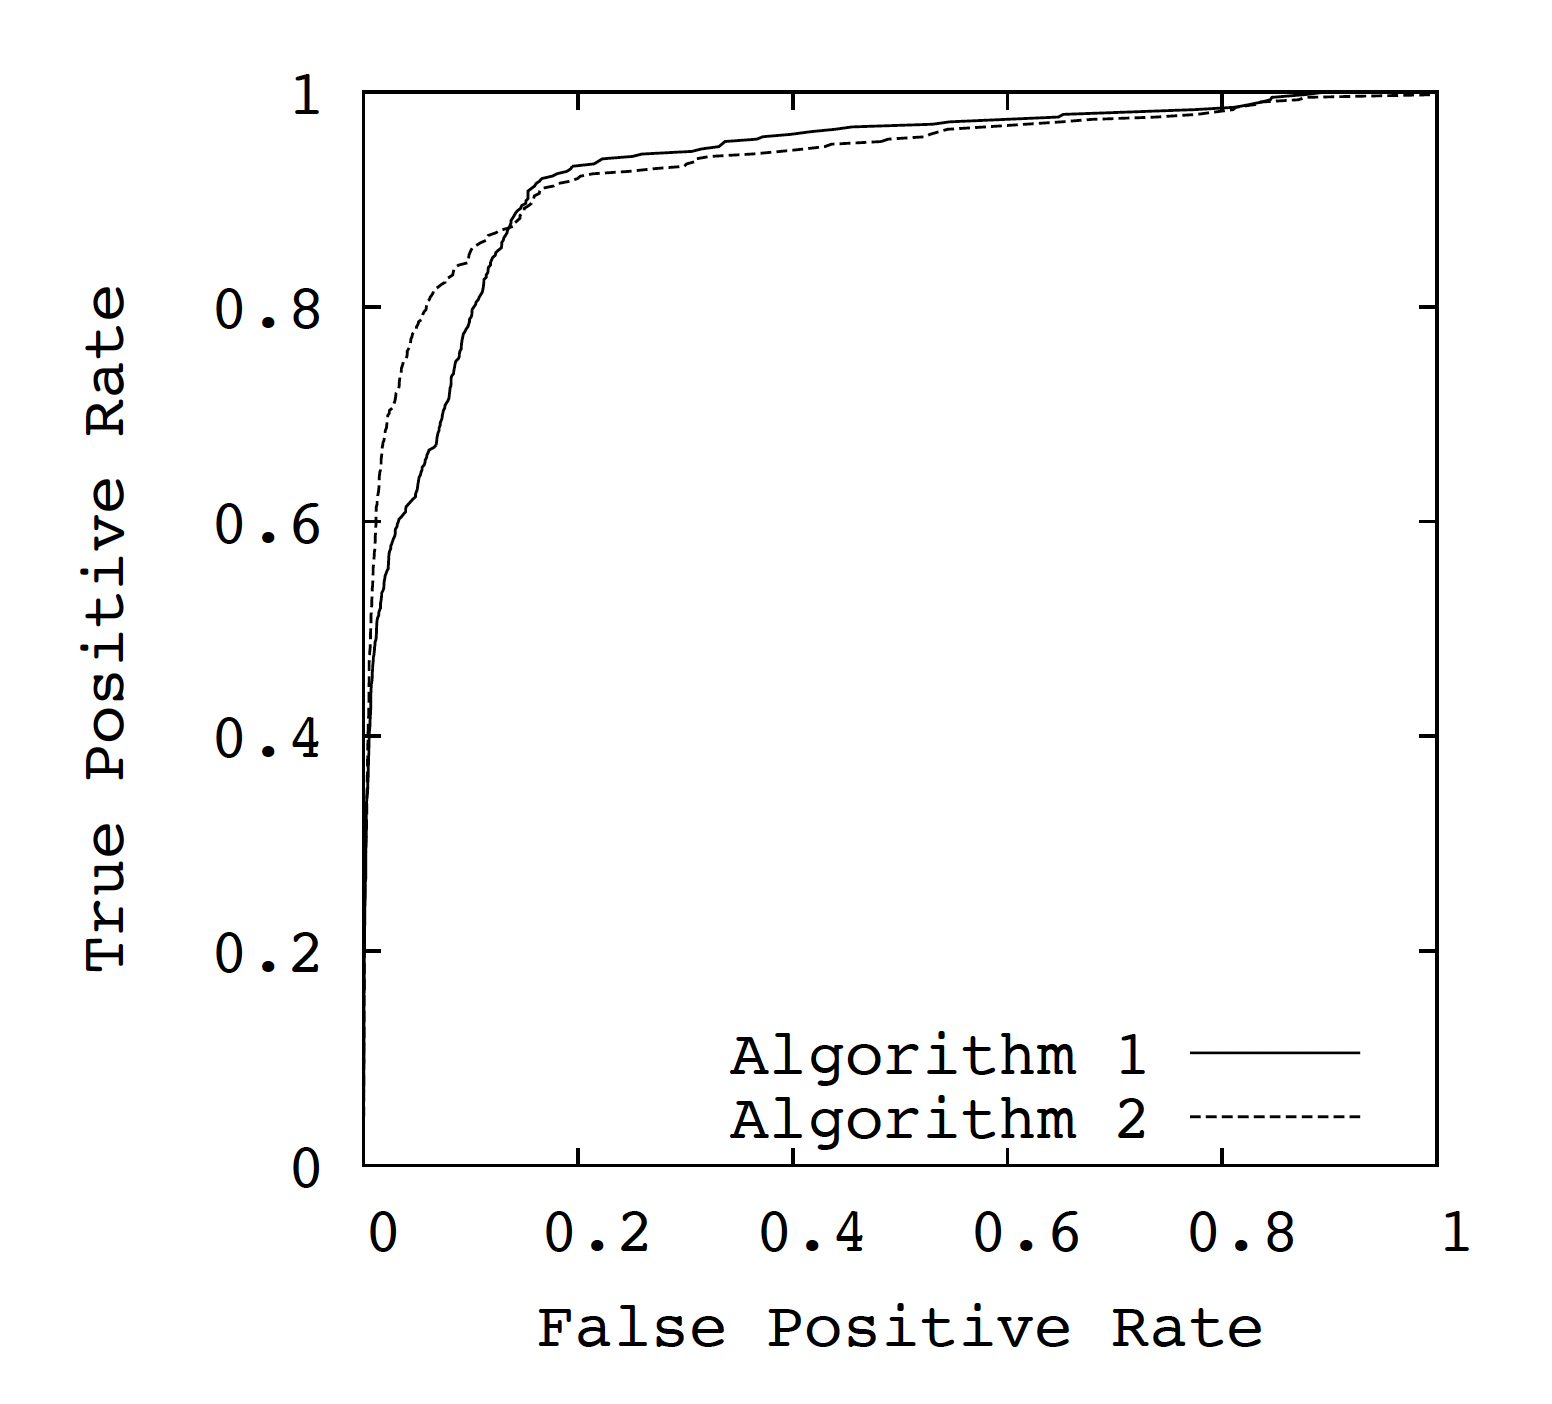
\includegraphics[width=.5\linewidth]{images/roc_curve}
    \caption{ROC Curve example\label{fig:ROC-curve}}
\end{figure}

Through a collaboration with Dr.~Fei-Fei Liu, head of the Radiation Medicine Program at Princess
Margaret Cancer Centre, prof. Benjamin Haibe-Kains has access to a unique set of \~500 scans of
head-and-neck cancer patients with associated survival data. The goal of this project is to develop
a new deep learning framework to analyze this private dataset in combination with public databases
to improve the prediction rate of patients' survival compared to models built on traditional 
radiomic features. Two of the methods that will be explored are dropout and image augmentation 
techniques to improve the fitting of neural networks from medical images. 

\subsection{Stakeholders}

\subsubsection{Developer}
\subsubsection{Physicians and Hospitals}
\subsubsection{Patients}

\section{State-of-the-art}

\section{Scope}

\pagebreak
\printbibliography{}

\end{document}